\section{\ifCDLeng Content\fi \ifCDLita Contenuto\fi}

\subsection{\ifCDLeng Notation\fi \ifCDLita Notazioni\fi}

\begin{Defn}
  \label{defn:1}
  \CDLeng Some definitions, $\cos(x)$ and \(\sin(x)\) are,
  \CDLeng for \(x\in\reals\),
  \CDLita Alcune definizioni $\cos(x)$ e \(\sin(x)\) sono,
  \CDLita per \(x\in\reals\),
  \index{$sin$@$\sin$}
  \index{$cos$@$\cos$}
  \indexLita{tangente|see{$\tan$}}
  \indexLita{$\tan$|see{tangente}}
  \indexLeng{tangent|see{$\tan$}}
  \indexLeng{$\tan$|see{tangent}}
  \begin{eqnarray}
    \CDLeng \tan(x)~, \label{english_only}\\
    \cos(x) \doteq \frac{e^{ix}+e^{-ix}}{2}~,  \label{eq:fefwe} \\
    \sin(x) \doteq \frac{e^{ix}-e^{-ix}}{2i}~. \label{eq:fefwe2}
  \end{eqnarray}
  \CDLeng A reference to a figure \ref{fig:a354}.
  \CDLita Un riferimento alla figura   \ref{fig:a354}.
  %
  \CDLeng A reference \eqref{eq:fefwe} and  \eqref{eq:fefwe2} to the above equations.
  \CDLita Un riferimento a \eqref{eq:fefwe} e  \eqref{eq:fefwe2} nelle equazioni precedenti.
\end{Defn}

\CDLeng A reference \eqref{english_only},\eqref{eq:fefwe} and  \eqref{eq:fefwe2} to the above equations.
\CDLita Un riferimento a \eqref{eq:fefwe} e  \eqref{eq:fefwe2} nelle equazioni precedenti.


\begin{figure}[ht]\label{fig:a354}
  \begin{center}
    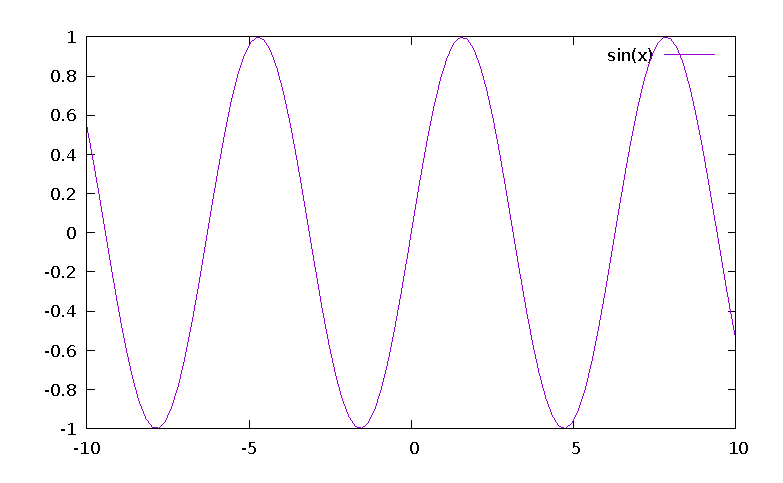
\includegraphics[width=0.5\textwidth]{F/sin}
    \caption{Graph of \(\sin(x)\).}
  \end{center}
\end{figure}




%%% Local Variables:
%%% mode: latex
%%% TeX-master: "paper"
%%% TeX-engine: xetex
%%% End:
